\chapter{Реализация}

\begin{figure}[h]
	\centering
	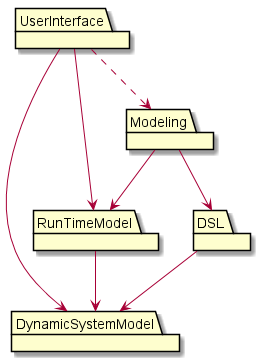
\includegraphics[width=0.5\linewidth]{package-diagram}
	\caption{Общая структура программного комплекса.\\Обычные стрелки --- явные зависимости.\\Пунктирные --- неявные.}
	\label{fig:package-diagram}
\end{figure}
\FloatBarrier
Исходя из требований, описанных в главе 2, можно выделить следующие библиотеки в программном комплексе (рис. \ref{fig:package-diagram}).
\begin{itemize}
	\item DynamicSystemModel~--- модель данных динамической системы. Содержит типы данных, описывающие структуру вычислительной сети.
	\item DSL~--- предметно-ориентированный язык и инструменты работы с языком, необходимые для преобразования исходного кода описания системы в модель данных.
	\item RunTimeModel~--- модель данных процесса моделирования. Содержит типы данных, необходимые для обмена информацией и исполнении команд модуля визуализации и управляющей программы.
	\item Modeling~--- управляющая программа, производящая моделирование и сбор данных об исполнении программы.
	\item UserInterface~--- модуль визуализации. 
	На схеме представлен, как один компонент, однако может быть представлен группой схожих компонентов, построенных на основе пакетов с моделями данных. 
	Ввиду того, что Kotlin позволяет создавать мультиплатформенные программы, описанные в пакетах моделей данных классы могут быть скомпилированы и использоваться в различных языках при условии использования только классов и структур данных, входящих в стандартную библиотеку Kotlin. 
	Это позволит иметь единую базу исходных кодов для реализаций клиентского приложения для различных платформ: браузеров, оконных приложений на Java или Kotlin, оконных приложений на C++, интерфейса командной строки, а также для интеграции с другим ПО.
\end{itemize}

Такая архитектура обособляет данные и способы взаимодействия с ними, что позволяет разделить приложение на слои и обеспечить максимально низкую зависимость слоёв друг от друга.
При подобном разбиении также облегчена задача обмена данными между сообщающимися модулями, т.к. они используют единый способ представления данных.

\section{Модель данных для описания системы}
Содержание пакета DynamicSystemModel изображено на рисунке \ref{fig:datamodel} и основано на описании формализма из главы 1.
Фундаментальным для системы является представление времени.
Особенность этого типа данных заключается в том, что областью значений для него является множество рациональных чисел в промежутке $ [0,\infty) $ объединённое с отдельно отстоящим значением $ \omega = \infty $.
При этом предполагается, что пользователь библиотеки не должен иметь возможность создавать собственные реализации класса \textit{Time}.
Продемонстрируем, как можно использовать Kotlin для решения данной задачи.

В Kotlin на уровне языка добавлена поддержка некоторых шаблонов проектирования, что существенно упрощает разработку.
Для ограничения возможности создавать реализации некоторого класса, его можно объявить изолированным, используя директиву \textbf{sealed} \cite{samuel2017programming}.
В таком случае наследников класса можно определить исключительно вложенными (nested) в класс-родитель.
На рисунке \ref{fig:sealed-class} изображен пример использования шаблона.

\begin{figure*}[h]
	\centering
	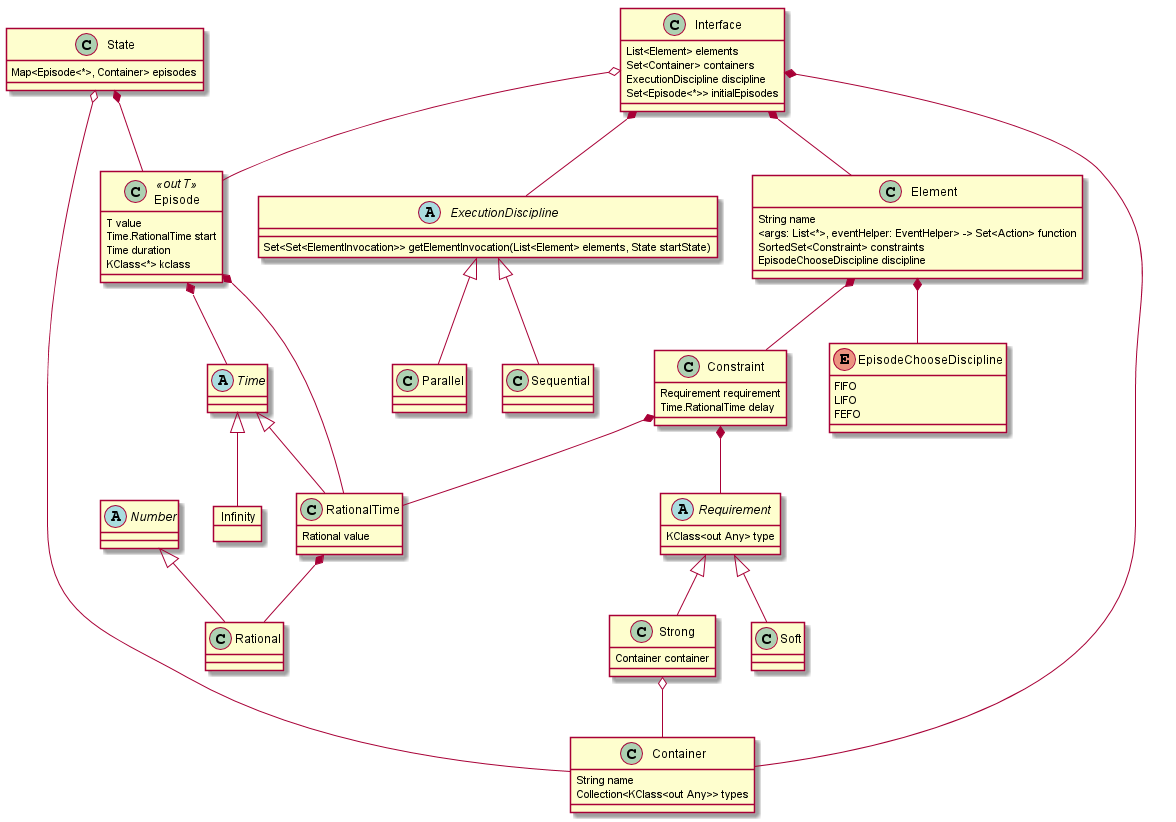
\includegraphics[width=0.9\linewidth]{images/datamodel}
	\caption{Модель данных динамической системы}
	\label{fig:datamodel}
\end{figure*}

\begin{figure*}[h]
	\centering
	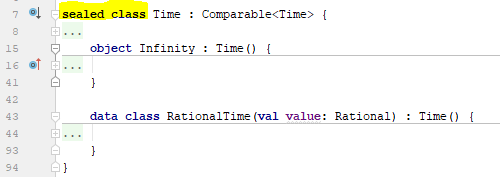
\includegraphics[width=0.7\linewidth]{images/sealed-class}
	\caption{Пример: Изолированный класс}
	\label{fig:sealed-class}
\end{figure*}
\FloatBarrier

Другим вспомогательным шаблоном, адаптированом в языке, является шаблон <<Одиночка>> (Singleton) \cite{morton1992object}. 
Он позволяет определить класс, для которого возможно наличие лишь одного экземпляра.
Таким классом является подкласс класса \textit{Time} - \textit{Infinity}.
На рисунке \ref{fig:object} изображено использование шаблона <<одиночка>>.
\begin{figure*}[h]
	\centering
	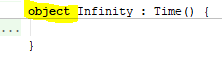
\includegraphics[width=0.4\linewidth]{images/object}
	\caption{Пример: Одиночка}
	\label{fig:object}
\end{figure*}
\FloatBarrier

Для работы с рациональными числами, исходя из описания шкалы времени в секции \ref{sec:time}, требуется их представление в виде упорядоченных пар целых чисел, а также определение указанных арифметических операций и отношений $ <, \leq, =, \geq, > $. 
Более того, желательно осуществлять приведения определённых пользователем чисел к каноническому виду. 
Для этих целей использована библиотека \textit{rational} \cite{Fylipp2018rational}.  
Она удовлетворяет всем выше указанным требованиям.
Пример её использования представлен в листинге \ref{list:rational}.

\lstinputlisting[lastline=78,language={Kotlin},caption={Пример использования библиотеки \textit{rational} для представления рациональных чисел.},label={list:rational}]{listings/rational.kt}

Для построения дерева процессов создан одиночка Modeler. Класс Modeler реализует алгоритм моделирования процесса.

\section{Модель данных процесса моделирования}


\begin{figure*}[h]
	\centering
	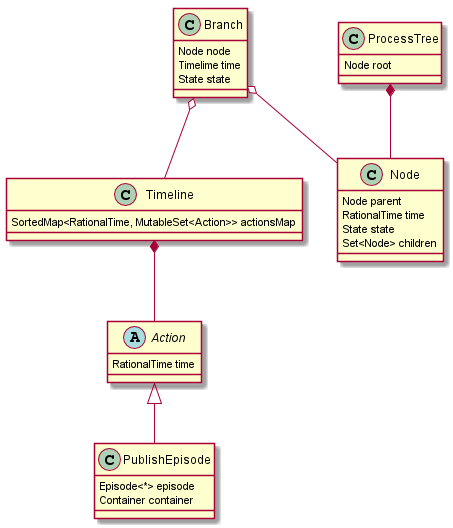
\includegraphics[width=0.7\linewidth]{images/runtimemodel}
	\caption{Модель данных процесса в динамической системе}
	\label{fig:runtimemodel}
\end{figure*}

На рисунке \ref{fig:runtimemodel} представлена модель данных процесса моделирования.
В соответствии с описанием из главы 1, процесс представлен в виде дерева \textit{ProcessTree}.
Для реализации построения такого дерева введено понятия графика событий (\textit{Timeline}).
Он представляет собой множество событий (\textit{Action}), сгруппированных по времени срабатывания. 
В данной программе реализовано событие появления нового эпизода в контейнере.

Исходя из определенного выше принципа ветвления дерева процесса следует, что описанная структура процесса является структурой ветвящегося в будущем времени \cite{ben1983temporal}. 
Следовательно, при итеративном моделировании процесса необходимо с каждым новым состоянием ассоциировать график событий, следующих за фиксацией нового состояния. 
Для этого создан класс \textit{Branch}.

\section{Предметно-ориентированный язык}
Целевой предметно-ориентированный язык должен позволять описать систему в начальный момент времени. 
Для этого необходимо реализовать определение эпизодов, содержащих эпизоды контейнеров, элементов интерфейса и их ограничений на входные эпизоды.

Помимо информационного атрибута, эпизоды в исходном состоянии системы могут отличаться длительностью. Примеры определения эпизодов представлены в листинге \ref{list:episode}. 
Т.к. Kotlin позволяет выводить типы переменных во время компиляции, не будем требовать явного указания типа данных для упрощения записи.
В случае, если длительность не указана, эпизод считается неограниченным по длительности.

\lstinputlisting[lastline=78,language={Kotlin},caption={DSL. Определение эпизода.},label={list:episode}]{listings/episode.kt}

Контейнер, в свою очередь, определяется уникальным именем и допустимыми сортами данных содержащихся в них эпизодов. Пример представлен в листинге \ref{list:container}. 
Для связи эпизодов с контейнером предлагается описывать эпизоды исключительно внутри декларации контейнера, как это показано на третьем примере в листинге.

\lstinputlisting[lastline=78,language={Kotlin},caption={DSL. Определение контейнера.},label={list:container}]{listings/container.kt}

Для определения элемента необходимо указать его требования к входным эпизодам, а также функцию, создающую новые эпизоды в системе.
Требования бывают двух типов. Мягкие требования определяются сортом данных требуемого эпизода и временем <<задержки>> на передачу эпизода в функцию. 
Жёсткое требование, в добавок к предыдущим параметрам, требует спецификации контейнера, в котором должен находиться целевой эпизод. Пример декларации требований описаны в листинге \ref{list:constraint}.

\lstinputlisting[lastline=78,language={Kotlin},caption={DSL. Требования к входным эпизодам элемента интерфейса.},label={list:constraint}]{listings/constraint.kt}

Определение элемента интерфейса приведено в листинге \ref{list:element}. 
Особое внимание следует уделить определению функции функционального базиса.
В качестве первого параметра она должна принимать список информационных атрибутов эпизодов, согласованных по порядку с порядком описания требований ко входным эпизодам.
Вторым параметром является вспомогательный объект, инкапсулирующий в себе создание новых эпизодов.
Результатом функции является множество новых событий о добавлении эпизодов.
Особенность DSL в Kotlin заключается в том, что такой DSL является библиотекой языка Kotlin и может использовать директивы языка. 
Благодаря этому в функции элемента интерфейса возможны любые выражения, допустимые в языке.

\lstinputlisting[lastline=78, language={Kotlin}, caption={DSL. Элемент интерфейса.}, label={list:element}] {listings/element.kt}

Исходя из описанного выше дизайна языка, можно составить способ определения исходного состояния системы на примере листинга \ref{list:interface}.
В нём описана простая система с тремя контейнерами.
Единственный элемент интерфейса выполняет конкатенацию информационных атрибутов двух входных строк и отправляет результат в контейнер результатов.
В результате выполнения такой программы в контейнере \textit{result} должен появиться эпизод со строкой \textit{<<Hello World!>>}.

\lstinputlisting[lastline=78, language={Kotlin}, caption={DSL. Определение исходного состояния системы.}, label={list:interface}] {listings/interface.kt}


\section{Визуализация}

Для визуализации полученного при моделировании графа решено использовать язык PlantUML \cite{plantuml2018Guide}.
PlantUML - проект с открытым исходным кодом, позволяющий быстро создавать диаграмы, используя простой и интуитивно понятный язык.
В данной работе построено отображение модели данных динамических систем в язык PlantUML. 
Исходный код для такого преобразования представлен в листинге \ref{list:plantuml}.

Пример из листинга \ref{list:interface} в отображении на PlantUML в текстовом виде приведён в листинге \ref{list:puml}, а визуализация примера изображена на рисунке 

\lstinputlisting[lastline=78, caption={Описание примера из листинга \ref{list:interface} на PlantUML.}, label={list:puml}] {listings/state0.puml}

\begin{figure*}[h]
	\centering
	\includegraphics[width=0.7\linewidth]{state0}
	\caption{Визуализация примера из листинга \ref{list:interface}.}
	\label{fig:interface}
\end{figure*}

Визуализация процесса для этого примера приведена в приложении \ref{AppendixA}.

В приложении \ref{AppendixB} показана реализация алгоритма Евклида, а также проведена симуляция процесса.

%\section{Тестирование}



%\begin{figure*}[h]
%	\centering
%	\includegraphics[width=0.7\linewidth]{images/state0}
%	\caption{Визуализация примера из листинга \ref{list:interface}. Состояние 1.}
%	\label{fig:state1}
%\end{figure*}
%\begin{figure*}[h]
%	\centering
%	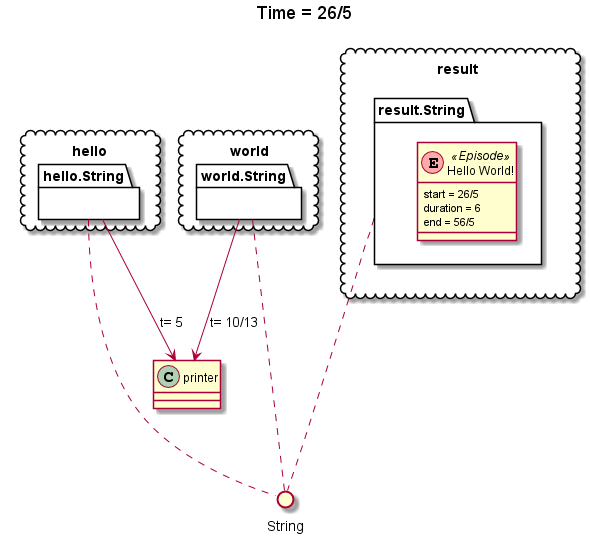
\includegraphics[width=0.7\linewidth]{images/state1}
%	\caption{Визуализация примера из листинга \ref{list:interface}. Состояние 2.}
%	\label{fig:state2}
%\end{figure*}
%
%
%%\section{Пример работы}
%\begin{figure*}[h]
%	\centering
%	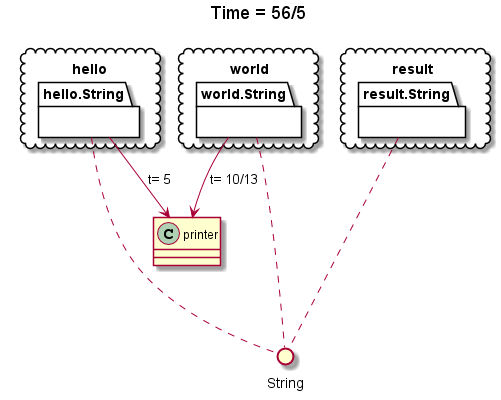
\includegraphics[width=0.7\linewidth]{images/state2}
%	\caption{{Визуализация примера из листинга \ref{list:interface}. Состояние 3.}
%	\label{fig:state3}
%\end{figure*}

